%versi 2 (8-10-2016) 
\chapter{Pendahuluan}
\label{chap:intro}
   
\section{Latar Belakang}
\label{sec:label}

Perkembangan teknologi pembuatan \web telah mengalami perubahan yang sangat pesat dalam 5 tahun terakhir. Sejak kemunculannya, \web telah menjadi platform utama dalam penyebaran informasi, komunikasi, hingga transaksi digital. Seiring meningkatnya kebutuhan pengguna terhadap kecepatan, keamanan, dan interaktivitas, berbagai teknologi baru terus bermunculan untuk mendukung pengembangan \web yang lebih efisien dan responsif.

Internet sendiri merupakan jaringan yang menghubungkan berbagai perangkat untuk memungkinkan pertukaran informasi secara cepat. Pertukaran informasi ini diatur oleh protokol utama TCP/IP (\textit{Transmission Control Protocol/Internet Protocol}). Namun, informasi yang dikirimkan di internet harus mudah dipahami oleh pengguna, tidak hanya dalam bentuk teks tetapi juga melalui gambar, video, dan suara. Kebutuhan inilah yang mendorong berkembangnya layanan \web (\textit{World Wide \web}), yang memungkinkan penyajian informasi secara lebih interaktif dengan memanfaatkan protokol HTTP (\textit{HyperText Transfer Protocol}).

Teknologi pembuatan \web semakin beragam dalam perkembangannya, baik dari sisi \textit{front-end} maupun \textit{back-end}. Beberapa teknologi utama yang mendukung pengembangan \web di antaranya adalah JavaScript, PHP, dan MySQL. Munculnya berbagai \textit{framework} dan pustaka seperti React, Vue.js, dan Node.js juga mempercepat adopsi teknologi baru dalam pengembangan \web modern. Perubahan ini membuat pentingnya pemantauan tren teknologi \web agar pengembang dapat memilih teknologi yang sesuai dengan kebutuhan pengguna dan standar industri.

Situs \textit{HTTP Archive} menyediakan data tentang teknologi yang digunakan dalam pembuatan \web untuk mencatat perkembangan teknologi ini. Situs ini mengumpulkan data berdasarkan berbagai aspek, seperti pengalaman pengguna dalam mengakses \web, kecepatan pemuatan halaman, serta tingkat aksesibilitas. Salah satu aspek utama yang diamati dalam penelitian ini adalah \textit{Chrome User Experience Report} (CrUX), yang mengukur tingkat interaktivitas dan kecepatan pemuatan \web berdasarkan data nyata dari pengguna peramban Google Chrome.

Data dari \textit{HTTP Archive} kemudian disimpan dalam \textit{Google BigQuery}, layanan penyimpanan dan analisis data berbasis \textit{cloud} yang memungkinkan pemrosesan data dalam skala besar menggunakan \textit{query SQL}. Dengan adanya teknologi ini, analisis terhadap perkembangan teknologi pembuatan \web dapat dilakukan secara lebih mendalam dan berbasis data yang akurat.

Untuk mempermudah pemahaman terhadap hasil analisis, penelitian ini akan menggunakan visualisasi data dalam bentuk grafik. Salah satu bentuk visualisasi yang digunakan adalah \textit{line chart}, yang dapat menunjukkan tren perubahan teknologi dalam rentang waktu tertentu secara lebih jelas. Contoh \textit{line chart} dapat dilihat pada gambar~\ref{fig:contohlinechart}\footnote{Gambar didapatkan dari \url{https://www.simonsezit.com/article/how-to-make-a-line-graph-in-excel/}}. Perkembangan penggunaan berbagai teknologi \web dapat divisualisasikan sehingga pola-pola perubahan dapat dikenali dengan lebih mudah dengan menggunakan \textit{line chart}. Selain itu, bentuk visualisasi lainnya seperti \textit{bar chart} dan \textit{scatter plot} juga odigunakan untuk memberikan perspektif tambahan terhadap data yang dianalisis.

\begin{figure}[]
        \centering
        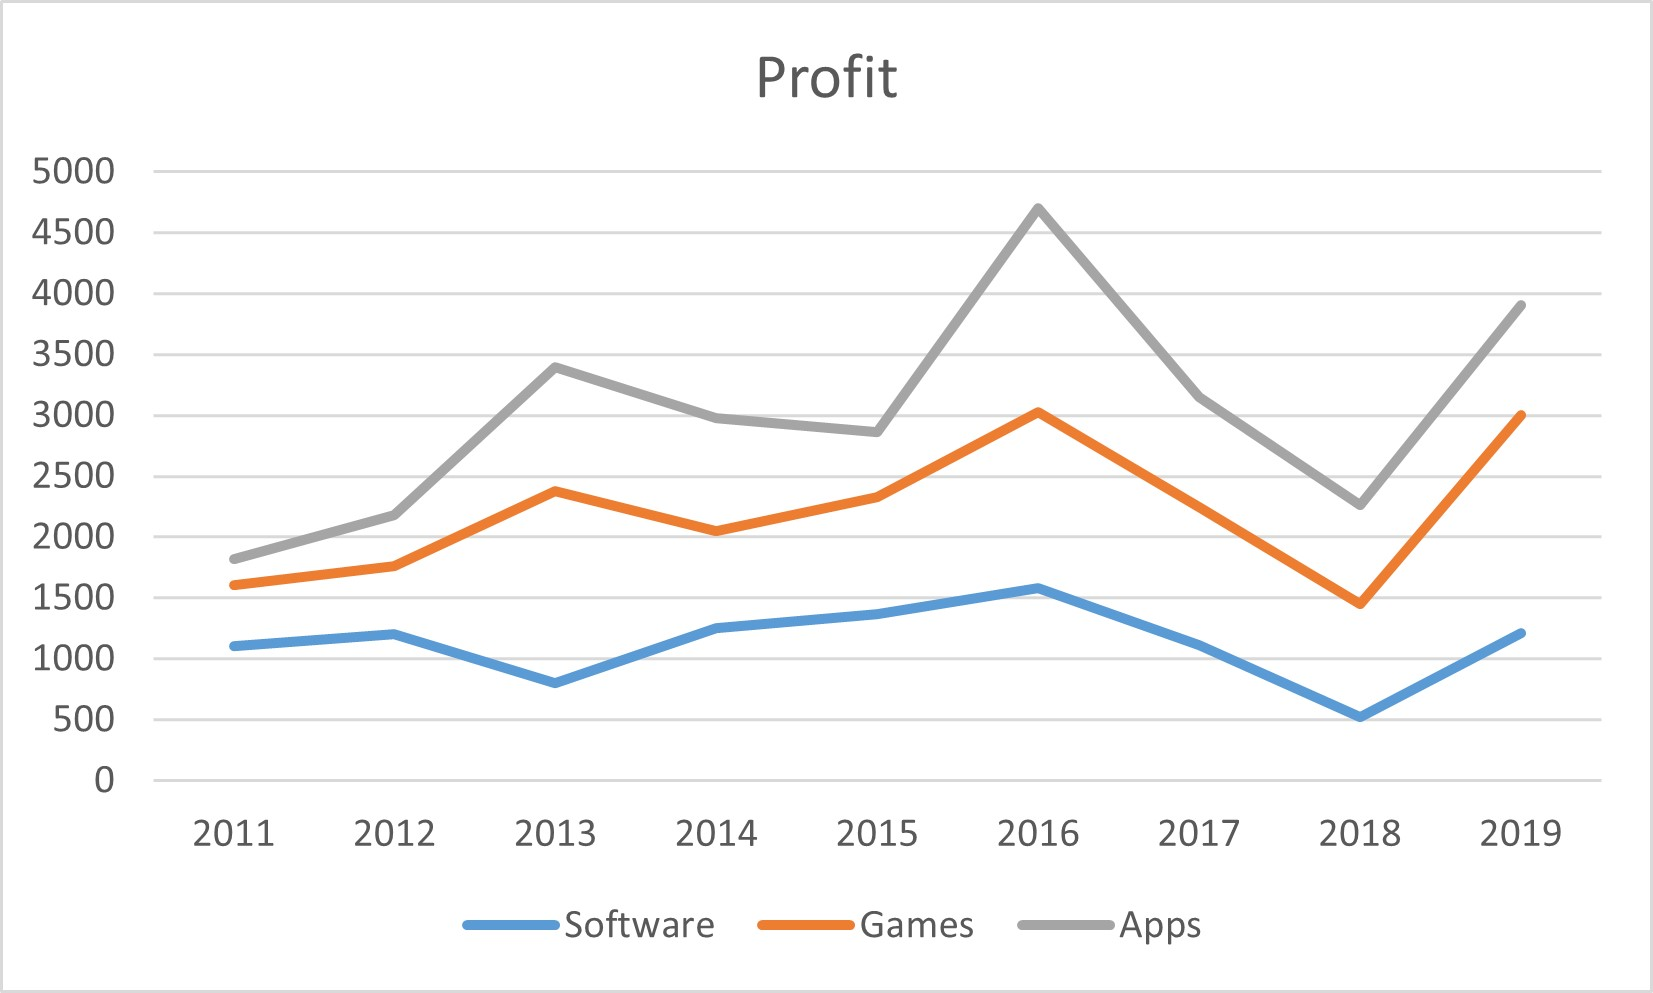
\includegraphics[width=0.5\linewidth]{Gambar/contoh linechart.jpg}
        \caption{Contoh \textit{line chart}}
        \label{fig:contohlinechart}
    \end{figure}

Penelitian ini bertujuan untuk memahami bagaimana tren teknologi pembuatan \web berkembang dalam 5 tahun terakhir, dari Oktober 2018 hingga Desember 2024. Dengan menggunakan data dari \textit{HTTP Archive} dan \textit{Google BigQuery}, penelitian ini akan mengeksplorasi perubahan signifikan dalam penggunaan teknologi \web dan dampaknya terhadap pengalaman pengguna. Hasil analisis ini diharapkan dapat memberikan wawasan bagi pengembang \web dan industri teknologi dalam memahami arah perkembangan \web di masa depan.
    
\section{Rumusan Masalah}
	Rumusan masalah yang akan diselesaikan dalam penelitian ini adalah:
    \begin{enumerate}
        \item Bagaimana perkembangan teknologi pembuatan \web selama 5 tahun terakhir?
        \item Bagaimana pekembangan teknologi pembuatan \web yang banyak digunakan oleh pembuat \web?
        \item Bagaimana cara menyajikan pekembangan teknologi pembuatan \web kepada pengguna?
    \end{enumerate}
	
\section{Tujuan}
	Tujuan yang akan dicapai dari penelitian ini adalah:
    \begin{enumerate}
        \item Mengetahui perkembangan teknologi pembuatan \web selama 5 tahun terakhir.
        \item Mengetahui perkembangan teknologi pembuatan \web yang banyak digunakan oleh pembuat \web.
        \item Membuat perangkat lunak untuk menyajikan perkembangan teknologi pembuatan \web.
    \end{enumerate}
\section{Batasan Masalah}
\label{sec:batasan}
Batasan masalah yang diterapkan pada penelitian ini adalah sebagai berikut:
\begin{enumerate}
    \item Data yang digunakan berasal dari rentang 5 tahun terkahir. Hal ini dimaksudkan untuk membatasi ukuran data agar tidak besar.
    \item Data yang akan dianalisis adalah data jumlah penggunaan dan persentase penggunaan. Hal ini dilakukan agar cakupan analisis tidak terlalu besar.
\end{enumerate}

\section{Metodologi}
\label{sec:metlit}
Metodologi yang digunakan dalam melakukan penelitian ini adalah sebagai berikut:
\begin{itemize}
    \item Mengumpulkan data penggunaan teknologi pembuatan \web selama 5 tahun terakhir.
    \item Membersihkan data dari kolom dan baris yang tidak digunakan.
    \item Melakukan analisis dengan menggunakan data dengan skala lebih kecil.
    \item Melakukan analisis dengan menggunakan data yang sebenarnya.
    \item Membuat perangkat lunak untuk menampilkan hasil analisis secara interaktif.
\end{itemize}

\section{Sistematika Pembahasan}
\label{sec:sispem}
Sistematika pembahasan tugas akhir ini adalah:
\begin{enumerate}
    \item Bab 1: Pendahuluan
   
    Membahas latar belakang, tujuan, rumusan masalah, batasan masalah, dan metodologi penelitian yang digunakan.
    
    \item Bab 2: Landasan Teori

    Membahas \web, \textit{HTTP Archive}, bahasa SQL, \textit{Google Big Query}, dan visualisasi data yang digunakan.

    \item Bab 3: Analisis Masalah

    Membahas tentang analisis masalah dan solusinya dan melakukan analisis dengan menggunakan data yang skalanya lebih kecil.

    \item Bab 4: Penambangan Data
    
    Membahas eksplorasi dan analisis data dengan menggunakan data \textit{real}.

    \item Bab 5: Pembuatan perangkat lunak dan Peluncuran Model

    Membahas tentang pembuatan perangkat lunak dan pengujian fungsional perangkat lunak untuk menampilkan hasil anlisis secara interaktif.

    \item Bab 6 : Kesimpulan dan Saran

    Membahas tentang kesimpulan dari hasil penelitian yang telah dilakukan dan saran agar peelitian ini lebih baik.
\end{enumerate}
